\documentclass[]{article}
\usepackage{lmodern}
\usepackage{amssymb,amsmath}
\usepackage{ifxetex,ifluatex}
\usepackage{fixltx2e} % provides \textsubscript
\ifnum 0\ifxetex 1\fi\ifluatex 1\fi=0 % if pdftex
  \usepackage[T1]{fontenc}
  \usepackage[utf8]{inputenc}
\else % if luatex or xelatex
  \ifxetex
    \usepackage{mathspec}
  \else
    \usepackage{fontspec}
  \fi
  \defaultfontfeatures{Ligatures=TeX,Scale=MatchLowercase}
\fi
% use upquote if available, for straight quotes in verbatim environments
\IfFileExists{upquote.sty}{\usepackage{upquote}}{}
% use microtype if available
\IfFileExists{microtype.sty}{%
\usepackage{microtype}
\UseMicrotypeSet[protrusion]{basicmath} % disable protrusion for tt fonts
}{}
\usepackage[margin=1in]{geometry}
\usepackage{hyperref}
\hypersetup{unicode=true,
            pdfborder={0 0 0},
            breaklinks=true}
\urlstyle{same}  % don't use monospace font for urls
\usepackage{color}
\usepackage{fancyvrb}
\newcommand{\VerbBar}{|}
\newcommand{\VERB}{\Verb[commandchars=\\\{\}]}
\DefineVerbatimEnvironment{Highlighting}{Verbatim}{commandchars=\\\{\}}
% Add ',fontsize=\small' for more characters per line
\usepackage{framed}
\definecolor{shadecolor}{RGB}{248,248,248}
\newenvironment{Shaded}{\begin{snugshade}}{\end{snugshade}}
\newcommand{\AlertTok}[1]{\textcolor[rgb]{0.94,0.16,0.16}{#1}}
\newcommand{\AnnotationTok}[1]{\textcolor[rgb]{0.56,0.35,0.01}{\textbf{\textit{#1}}}}
\newcommand{\AttributeTok}[1]{\textcolor[rgb]{0.77,0.63,0.00}{#1}}
\newcommand{\BaseNTok}[1]{\textcolor[rgb]{0.00,0.00,0.81}{#1}}
\newcommand{\BuiltInTok}[1]{#1}
\newcommand{\CharTok}[1]{\textcolor[rgb]{0.31,0.60,0.02}{#1}}
\newcommand{\CommentTok}[1]{\textcolor[rgb]{0.56,0.35,0.01}{\textit{#1}}}
\newcommand{\CommentVarTok}[1]{\textcolor[rgb]{0.56,0.35,0.01}{\textbf{\textit{#1}}}}
\newcommand{\ConstantTok}[1]{\textcolor[rgb]{0.00,0.00,0.00}{#1}}
\newcommand{\ControlFlowTok}[1]{\textcolor[rgb]{0.13,0.29,0.53}{\textbf{#1}}}
\newcommand{\DataTypeTok}[1]{\textcolor[rgb]{0.13,0.29,0.53}{#1}}
\newcommand{\DecValTok}[1]{\textcolor[rgb]{0.00,0.00,0.81}{#1}}
\newcommand{\DocumentationTok}[1]{\textcolor[rgb]{0.56,0.35,0.01}{\textbf{\textit{#1}}}}
\newcommand{\ErrorTok}[1]{\textcolor[rgb]{0.64,0.00,0.00}{\textbf{#1}}}
\newcommand{\ExtensionTok}[1]{#1}
\newcommand{\FloatTok}[1]{\textcolor[rgb]{0.00,0.00,0.81}{#1}}
\newcommand{\FunctionTok}[1]{\textcolor[rgb]{0.00,0.00,0.00}{#1}}
\newcommand{\ImportTok}[1]{#1}
\newcommand{\InformationTok}[1]{\textcolor[rgb]{0.56,0.35,0.01}{\textbf{\textit{#1}}}}
\newcommand{\KeywordTok}[1]{\textcolor[rgb]{0.13,0.29,0.53}{\textbf{#1}}}
\newcommand{\NormalTok}[1]{#1}
\newcommand{\OperatorTok}[1]{\textcolor[rgb]{0.81,0.36,0.00}{\textbf{#1}}}
\newcommand{\OtherTok}[1]{\textcolor[rgb]{0.56,0.35,0.01}{#1}}
\newcommand{\PreprocessorTok}[1]{\textcolor[rgb]{0.56,0.35,0.01}{\textit{#1}}}
\newcommand{\RegionMarkerTok}[1]{#1}
\newcommand{\SpecialCharTok}[1]{\textcolor[rgb]{0.00,0.00,0.00}{#1}}
\newcommand{\SpecialStringTok}[1]{\textcolor[rgb]{0.31,0.60,0.02}{#1}}
\newcommand{\StringTok}[1]{\textcolor[rgb]{0.31,0.60,0.02}{#1}}
\newcommand{\VariableTok}[1]{\textcolor[rgb]{0.00,0.00,0.00}{#1}}
\newcommand{\VerbatimStringTok}[1]{\textcolor[rgb]{0.31,0.60,0.02}{#1}}
\newcommand{\WarningTok}[1]{\textcolor[rgb]{0.56,0.35,0.01}{\textbf{\textit{#1}}}}
\usepackage{graphicx,grffile}
\makeatletter
\def\maxwidth{\ifdim\Gin@nat@width>\linewidth\linewidth\else\Gin@nat@width\fi}
\def\maxheight{\ifdim\Gin@nat@height>\textheight\textheight\else\Gin@nat@height\fi}
\makeatother
% Scale images if necessary, so that they will not overflow the page
% margins by default, and it is still possible to overwrite the defaults
% using explicit options in \includegraphics[width, height, ...]{}
\setkeys{Gin}{width=\maxwidth,height=\maxheight,keepaspectratio}
\IfFileExists{parskip.sty}{%
\usepackage{parskip}
}{% else
\setlength{\parindent}{0pt}
\setlength{\parskip}{6pt plus 2pt minus 1pt}
}
\setlength{\emergencystretch}{3em}  % prevent overfull lines
\providecommand{\tightlist}{%
  \setlength{\itemsep}{0pt}\setlength{\parskip}{0pt}}
\setcounter{secnumdepth}{0}
% Redefines (sub)paragraphs to behave more like sections
\ifx\paragraph\undefined\else
\let\oldparagraph\paragraph
\renewcommand{\paragraph}[1]{\oldparagraph{#1}\mbox{}}
\fi
\ifx\subparagraph\undefined\else
\let\oldsubparagraph\subparagraph
\renewcommand{\subparagraph}[1]{\oldsubparagraph{#1}\mbox{}}
\fi

%%% Use protect on footnotes to avoid problems with footnotes in titles
\let\rmarkdownfootnote\footnote%
\def\footnote{\protect\rmarkdownfootnote}

%%% Change title format to be more compact
\usepackage{titling}

% Create subtitle command for use in maketitle
\providecommand{\subtitle}[1]{
  \posttitle{
    \begin{center}\large#1\end{center}
    }
}

\setlength{\droptitle}{-2em}

  \title{}
    \pretitle{\vspace{\droptitle}}
  \posttitle{}
    \author{}
    \preauthor{}\postauthor{}
    \date{}
    \predate{}\postdate{}
  

\begin{document}

\begin{Shaded}
\begin{Highlighting}[]
\NormalTok{dados <-}\StringTok{ }\KeywordTok{read.delim2}\NormalTok{(}\StringTok{"D:/Google Drive/2 - Ufpb/P5/Econometria/Series/Dados/cap3.txt"}\NormalTok{, }\DataTypeTok{row.names=}\DecValTok{1}\NormalTok{)}
\NormalTok{dados}
\end{Highlighting}
\end{Shaded}

\begin{verbatim}
##                DE     FP   TD
## 1995.01  46331.44  78.13  7.9
## 1995.02  46818.79  77.68  8.9
## 1995.03  48113.47  81.66  9.2
## 1995.04  50658.81  83.38  9.4
## 1995.05  53979.63  87.56  9.2
## 1995.06  56569.92  88.76  9.1
## 1995.07  58557.33  89.14  9.1
## 1995.08  59466.12  89.20  8.8
## 1995.09  59253.58  86.66  9.0
## 1995.10  59891.43  90.13  9.0
## 1995.11  60450.73 102.35  9.1
## 1995.12  64266.65 124.97  8.7
## 1996.01  64902.72  96.41  8.5
## 1996.02  65233.10  95.03  9.1
## 1996.03  65267.82  93.05 10.1
## 1996.04  65114.54  91.85 11.0
## 1996.05  64692.97  93.87 10.8
## 1996.06  64510.54  94.97 10.7
## 1996.07  64278.98  97.10 10.3
## 1996.08  64236.00  97.83 10.3
## 1996.09  64726.91  97.61  9.9
## 1996.10  65754.07  97.14  9.7
## 1996.11  67558.05 108.59  9.6
## 1996.12  72652.00 138.35  9.2
## 1997.01  77130.33 101.62  8.9
## 1997.02  78711.82  97.11  9.1
## 1997.03  80034.28  98.39  9.9
## 1997.04  80883.31  98.20 10.7
## 1997.05  81791.65  98.25 10.7
## 1997.06  82927.44  98.67 10.5
## 1997.07  83626.27 100.64 10.2
## 1997.08  85063.78  98.10 10.2
## 1997.09  86591.73  97.79 10.5
## 1997.10  88145.78  97.99 10.5
## 1997.11  93941.90 110.44 10.5
## 1997.12  98211.26 136.19 10.2
## 1998.01 100628.94  99.99 10.3
## 1998.02  98600.98  95.68 11.1
## 1998.03  98108.16  94.76 12.0
## 1998.04  97850.78  93.11 12.5
## 1998.05  98234.21  95.42 12.4
## 1998.06  99703.66  94.21 12.3
## 1998.07 101146.46  93.65 12.1
## 1998.08 102317.11  91.50 12.0
## 1998.09 104162.81  89.41 11.7
## 1998.10 105773.76  90.39 11.6
## 1998.11 107168.49 100.64 11.3
## 1998.12 108442.38 122.15 10.8
## 1999.01 109360.15  89.15 10.7
## 1999.02 111432.30  84.90 11.6
## 1999.03 112363.68  86.10 12.9
## 1999.04 112524.50  85.04 13.4
## 1999.05 113364.45  86.34 12.9
## 1999.06 112787.04  86.06 12.5
## 1999.07 112300.92  86.51 12.6
## 1999.08 111709.81  85.77 12.4
## 1999.09 110964.42  85.78 12.2
## 1999.10 110498.34  87.34 11.6
## 1999.11 110695.59  99.49 11.4
## 1999.12 111406.67 123.45 10.5
## 2000.01 112685.74  94.76 10.6
## 2000.02 111879.54  92.27 10.5
## 2000.03 111304.74  91.54 11.3
## 2000.04 110935.78  90.22 11.8
## 2000.05 110441.69  91.48 11.8
## 2000.06 111044.99  91.89 11.7
## 2000.07 111006.66  93.66 11.6
## 2000.08 110716.14  91.95 11.2
## 2000.09 109494.43  90.94 11.0
## 2000.10 108731.59  93.37 10.4
## 2000.11 109260.19 105.32 10.3
## 2000.12 111936.10  91.87 10.0
## 2001.01 112272.26 100.00 10.1
## 2001.02 112831.87  98.43 10.7
## 2001.03 112398.66 109.13 11.2
## 2001.04 112749.02 116.22 11.5
## 2001.05 113891.73 109.82 11.0
## 2001.06 114874.37 108.84 10.7
## 2001.07 115508.72 109.21 10.9
## 2001.08 116060.60  85.80 11.3
## 2001.09 116737.77  98.42 11.5
## 2001.10 116399.42  89.49 11.9
## 2001.11 117676.13  99.62 11.7
## 2001.12 120030.42 129.37 11.6
## 2002.01 120034.06 114.40 11.3
## 2002.02 120495.52 104.33 12.0
## 2002.03 120786.60 133.33 12.8
## 2002.04 120419.32 140.31 13.3
## 2002.05 120908.90 127.01 12.8
## 2002.06 126974.87 127.69 12.0
## 2002.07 131996.17 122.69 11.5
## 2002.08 136876.68 101.35 11.8
## 2002.09 138721.22 117.96 12.2
## 2002.10 139529.47 122.05 12.3
## 2002.11 140309.02 105.99 12.0
## 2002.12 140895.70 120.41 11.4
## 2003.01 141282.81 123.67 11.2
## 2003.02 140814.92 133.24 11.9
## 2003.03 139704.83 150.89 12.7
## 2003.04 138719.21 158.07 13.6
## 2003.05 138432.05 144.76 13.4
## 2003.06 138247.44 146.91 13.2
## 2003.07 138812.24 131.20 12.7
## 2003.08 139451.14 104.52 12.9
## 2003.09 139195.38 133.82 13.2
## 2003.10 139129.36 118.14 13.2
## 2003.11 141200.60 120.50 12.6
## 2003.12 144118.43 135.72 12.0
## 2004.01 144683.60 140.33 11.9
## 2004.02 144902.04 133.84 12.6
## 2004.03 144291.74 203.70 13.3
## 2004.04 144734.92 200.19 13.2
## 2004.05 147287.54 181.74 12.3
## 2004.06 149287.47 194.60 11.8
## 2004.07 151502.62 184.17 11.7
## 2004.08 152155.18 177.55 11.7
## 2004.09 152920.90 182.48 11.4
## 2004.10 153680.11 146.46 10.8
## 2004.11 155244.31 153.20 10.4
## 2004.12 159588.79 180.94 10.0
## 2005.01 160218.69 162.33  9.9
## 2005.02 160232.29 147.92 10.4
## 2005.03 159708.51 206.63 10.9
## 2005.04 159438.24 217.23 11.1
## 2005.05 158834.89 207.72 11.0
## 2005.06 159920.73 218.92 11.0
## 2005.07 161792.50 205.04 10.8
## 2005.08 161674.96 191.45 10.6
## 2005.09 162195.29 194.85 10.4
## 2005.10 162628.36 183.98 10.6
## 2005.11 164240.58 161.03 10.2
## 2005.12 169322.67 249.09  9.7
## 2006.01 168740.22 169.70  9.5
## 2006.02 169964.48 171.42 10.2
## 2006.03 167242.33 203.62 10.9
## 2006.04 166661.12 240.09 11.2
## 2006.05 166049.30 191.14 11.3
## 2006.06 167620.32 207.15 11.3
## 2006.07 170109.60 207.24 11.3
## 2006.08 171003.43 179.66 10.7
## 2006.09 174233.25 196.67 10.3
## 2006.10 176209.35 145.95  9.6
## 2006.11 180118.52 157.65  9.1
## 2006.12 187864.03 168.26  9.0
## 2007.01 189734.96 134.61  9.0
## 2007.02 192044.83 154.41  9.7
## 2007.03 194873.23 170.74 10.4
## 2007.04 197639.65 185.45 10.9
## 2007.05 200246.41 194.50 10.6
## 2007.06 203955.12 209.24 10.3
## 2007.07 208214.26 182.30 10.5
## 2007.08 212971.47 161.37 10.4
## 2007.09 218432.22 175.34 10.5
## 2007.10 221168.74 127.57 10.0
## 2007.11 225354.95 177.32 10.0
## 2007.12 234671.90 177.59  9.3
## 2008.01 237490.43 206.24  9.3
## 2008.02 240438.78 194.59  9.1
## 2008.03 242582.02 183.04  9.6
## 2008.04 242699.02 191.40  9.8
## 2008.05 245170.73 191.35  9.8
## 2008.06 248087.17 207.95  9.7
## 2008.07 251930.71 191.00  9.6
## 2008.08 255225.91 178.19  9.4
## 2008.09 258397.67 182.31  9.3
## 2008.10 259940.52 135.49  8.5
## 2008.11 264128.86 158.49  8.6
## 2008.12 271156.74 193.53  8.3
## 2009.01 272499.57 176.17  9.2
## 2009.02 274852.75 218.35  9.8
## 2009.03 275496.47 181.89 10.8
## 2009.04 276043.85 204.07 10.9
## 2009.05 279463.48 214.00 10.8
## 2009.06 283038.10 218.60 10.3
## 2009.07 291041.25 216.45 10.5
## 2009.08 295603.41 189.22 10.1
## 2009.09 300498.35 209.01 10.1
## 2009.10 302983.25 162.13  9.9
## 2009.11 309223.99 178.04  9.4
## 2009.12 319631.93 203.48  8.5
## 2010.01 323908.66 188.85  8.0
## 2010.02 326604.36 210.78  8.5
## 2010.03 328636.03 204.89  9.6
## 2010.04 331852.08 215.87  9.8
## 2010.05 335901.45 218.60  9.7
## 2010.06 341889.87 231.48  9.5
## 2010.07 350691.95 224.49  9.4
## 2010.08 354495.99 221.02  9.3
## 2010.09 361242.17 202.28  8.7
## 2010.10 365719.67 163.69  8.4
## 2010.11 371209.62 179.90  8.1
## 2010.12 379604.27 200.02  7.4
## 2011.01 382043.99 182.74  8.0
## 2011.02 383334.10 217.67  8.1
## 2011.03 385733.26 187.75  9.0
## 2011.04 386122.94 212.34  8.8
## 2011.05 387046.56 217.92  8.5
## 2011.06 389558.70 225.61  8.7
## 2011.07 398005.68 229.46  8.8
## 2011.08 402719.24 231.55  9.0
## 2011.09 409310.51 208.51  8.5
## 2011.10 412717.60 176.73  7.9
## 2011.11 414983.46 188.02  7.5
## 2011.12 420872.65 250.40  6.9
## 2012.01 423261.83 200.01  7.6
## 2012.02 425054.07 232.69  8.4
## 2012.03 429860.85 221.77  9.1
## 2012.04 434077.04 222.80  9.1
## 2012.05 442527.44 237.71  8.8
## 2012.06 449801.59 234.92  9.0
## 2012.07 460241.95 240.25  9.1
## 2012.08 465932.01 219.67  9.4
## 2012.09 474052.53 223.85  9.1
## 2012.10 479470.97 177.87  8.5
## 2012.11 485716.89 209.88  7.9
## 2012.12 497139.07 271.25  7.6
## 2013.01 501669.86 249.95  7.8
## 2013.02 506417.66 235.02  8.2
## 2013.03 514654.97 229.65  8.8
## 2013.04 519548.89 248.45  9.1
## 2013.05 527860.46 246.30  9.0
## 2013.06 539315.24 256.53  9.1
## 2013.07 551158.75 275.61  9.0
## 2013.08 558449.22 254.85  8.6
## 2013.09 567882.04 311.47  8.1
## 2013.10 575369.02 195.33  7.7
## 2013.11 584781.09 233.07  7.5
## 2013.12 599825.99 259.37  7.5
## 2014.01 604824.60 314.94  7.8
## 2014.02 609877.47 254.36  8.7
## 2014.03 614875.53 470.16  9.4
## 2014.04 616830.71 255.57  9.6
## 2014.05 622339.69 256.64  9.5
## 2014.06 628926.42 265.61  9.4
## 2014.07 636446.77 288.60  9.4
## 2014.08 640564.03 274.37  9.2
## 2014.09 645474.10 307.97  8.7
## 2014.10 649650.21 208.17  8.1
## 2014.11 655806.26 237.50  7.9
## 2014.12 664847.30 236.60  8.0
## 2015.01 663517.45 258.53  7.9
## 2015.02 660210.26 255.43  8.7
## 2015.03 652549.19 382.40  9.4
## 2015.04 650444.73 295.58 10.2
## 2015.05 651079.30 263.25 10.7
## 2015.06 648879.27 267.99 11.1
## 2015.07 650714.09 297.03 11.4
## 2015.08 647539.58 263.54 11.5
## 2015.09 646378.45 281.29 11.8
## 2015.10 647197.56 218.67 11.9
## 2015.11 649996.77 227.97 11.7
## 2015.12 659005.51 237.94 11.5
## 2016.01 650996.72 263.54 11.8
## 2016.02 648289.78 281.29 12.3
## 2016.03 647003.07 218.67 13.4
## 2016.04 642773.09 227.97 14.2
## 2016.05 640246.59 237.94 15.0
## 2016.06 640680.04 263.54 14.7
## 2016.07 643807.20 281.29 14.2
## 2016.08 643658.87 218.67 13.9
## 2016.09 645433.35 227.97 14.4
## 2016.10 646800.71 237.94 14.3
## 2016.11 652682.55 263.54 14.0
## 2016.12 669286.30 281.29 13.5
## 2017.01 662201.48 218.67 14.1
## 2017.02 664105.90 227.97 14.8
## 2017.03 662919.50 229.65 15.2
## 2017.04 665181.33 255.57 15.5
## 2017.05 668998.34 256.64 15.9
## 2017.06 678744.38 265.61 15.6
## 2017.07 684707.83 288.60 15.1
## 2017.08 690409.72 281.29 14.5
## 2017.09 697406.90 218.67 14.5
## 2017.10 698581.33 227.97 14.8
## 2017.11 705588.13 237.94 14.1
## 2017.12 727981.35 263.54 12.9
## 2018.01 725734.25 281.29 13.2
## 2018.02 727848.59 218.67 13.6
## 2018.03 734825.27 281.29 14.5
## 2018.04 738795.11 218.67 14.4
## 2018.05 744039.51 227.97 14.2
## 2018.06 752524.35 229.65 14.1
## 2018.07 759125.38 227.97 14.6
## 2018.08 767980.28 237.94 14.4
## 2018.09 779246.72 263.54 13.9
## 2018.10 779696.01 281.29 13.1
## 2018.11 783382.48 293.53 12.4
## 2018.12 800889.43 296.36 12.5
\end{verbatim}

\begin{center}\rule{0.5\linewidth}{\linethickness}\end{center}

\#Modelo Naive

A previsão dele é igual ao valor da última observação ou quando há
sazonalidade, a previsão de um mês futuro é igual ao valor da última
observação.

\begin{Shaded}
\begin{Highlighting}[]
\KeywordTok{summary}\NormalTok{(}\KeywordTok{naive}\NormalTok{(dados[,}\DecValTok{1}\NormalTok{],}\DataTypeTok{h=}\DecValTok{27}\NormalTok{))}
\end{Highlighting}
\end{Shaded}

\begin{verbatim}
## 
## Forecast method: Naive method
## 
## Model Information:
## Call: naive(y = dados[, 1], h = 27) 
## 
## Residual sd: 3692.136 
## 
## Error measures:
##                    ME     RMSE      MAE       MPE     MAPE MASE      ACF1
## Training set 2629.122 4527.323 3137.336 0.9797526 1.165251    1 0.4537878
## 
## Forecasts:
##     Point Forecast    Lo 80    Hi 80    Lo 95    Hi 95
## 289       800889.4 795087.4 806691.4 792016.0 809762.8
## 290       800889.4 792684.2 809094.7 788340.6 813438.3
## 291       800889.4 790840.1 810938.8 785520.3 816258.6
## 292       800889.4 789285.4 812493.4 783142.7 818636.2
## 293       800889.4 787915.8 813863.1 781047.9 820730.9
## 294       800889.4 786677.5 815101.4 779154.2 822624.7
## 295       800889.4 785538.8 816240.1 777412.6 824366.2
## 296       800889.4 784478.9 817300.0 775791.7 825987.2
## 297       800889.4 783483.4 818295.4 774269.3 827509.6
## 298       800889.4 782541.9 819237.0 772829.3 828949.6
## 299       800889.4 781646.4 820132.5 771459.7 830319.1
## 300       800889.4 780790.7 820988.1 770151.1 831627.8
## 301       800889.4 779970.0 821808.8 768896.0 832882.9
## 302       800889.4 779180.3 822598.5 767688.2 834090.6
## 303       800889.4 778418.4 823360.5 766522.9 835255.9
## 304       800889.4 777681.4 824097.4 765395.9 836383.0
## 305       800889.4 776967.2 824811.7 764303.5 837475.4
## 306       800889.4 776273.6 825505.2 763242.8 838536.0
## 307       800889.4 775599.1 826179.8 762211.2 839567.6
## 308       800889.4 774942.1 826836.8 761206.4 840572.4
## 309       800889.4 774301.3 827477.5 760226.4 841552.4
## 310       800889.4 773675.6 828103.2 759269.5 842509.3
## 311       800889.4 773064.0 828714.8 758334.1 843444.7
## 312       800889.4 772465.6 829313.3 757418.9 844360.0
## 313       800889.4 771879.4 829899.4 756522.5 845256.4
## 314       800889.4 771304.9 830473.9 755643.8 846135.0
## 315       800889.4 770741.4 831037.5 754781.9 846996.9
\end{verbatim}

\begin{Shaded}
\begin{Highlighting}[]
\KeywordTok{summary}\NormalTok{(}\KeywordTok{naive}\NormalTok{(dados[,}\DecValTok{2}\NormalTok{],}\DataTypeTok{h=}\DecValTok{27}\NormalTok{))}
\end{Highlighting}
\end{Shaded}

\begin{verbatim}
## 
## Forecast method: Naive method
## 
## Model Information:
## Call: naive(y = dados[, 2], h = 27) 
## 
## Residual sd: 32.3072 
## 
## Error measures:
##                     ME     RMSE      MAE        MPE     MAPE MASE
## Training set 0.7603833 32.25986 19.28512 -0.5905468 10.17468    1
##                    ACF1
## Training set -0.4613094
## 
## Forecasts:
##     Point Forecast     Lo 80    Hi 80       Lo 95    Hi 95
## 289         296.36 255.01733 337.7027 233.1318401 359.5882
## 290         296.36 237.89263 354.8274 206.9418787 385.7781
## 291         296.36 224.75239 367.9676 186.8456145 405.8744
## 292         296.36 213.67466 379.0453 169.9036801 422.8163
## 293         296.36 203.91498 388.8050 154.9775363 437.7425
## 294         296.36 195.09155 397.6285 141.4832708 451.2367
## 295         296.36 186.97757 405.7424 129.0740129 463.6460
## 296         296.36 179.42527 413.2947 117.5237574 475.1962
## 297         296.36 172.33199 420.3880 106.6755202 486.0445
## 298         296.36 165.62299 427.0970  96.4150023 496.3050
## 299         296.36 159.24187 433.4781  86.6559173 506.0641
## 300         296.36 153.14478 439.5752  77.3312290 515.3888
## 301         296.36 147.29688 445.4231  68.3876273 524.3324
## 302         296.36 141.66989 451.0501  59.7818883 532.9381
## 303         296.36 136.24052 456.4795  51.4783895 541.2416
## 304         296.36 130.98931 461.7307  43.4473602 549.2726
## 305         296.36 125.89980 466.8202  35.6636180 557.0564
## 306         296.36 120.95790 471.7621  28.1056360 564.6144
## 307         296.36 116.15147 476.5685  20.7548404 571.9652
## 308         296.36 111.46995 481.2500  13.5950725 579.1249
## 309         296.36 106.90408 485.8159   6.6121710 586.1078
## 310         296.36 102.44568 490.2743  -0.2063579 592.9264
## 311         296.36  98.08751 494.6325  -6.8716026 599.5916
## 312         296.36  93.82310 498.8969 -13.3934585 606.1135
## 313         296.36  89.64664 503.0734 -19.7807997 612.5008
## 314         296.36  85.55291 507.1671 -26.0416214 618.7616
## 315         296.36  81.53718 511.1828 -32.1831565 624.9032
\end{verbatim}

\begin{Shaded}
\begin{Highlighting}[]
\KeywordTok{summary}\NormalTok{(}\KeywordTok{naive}\NormalTok{(dados[,}\DecValTok{3}\NormalTok{],}\DataTypeTok{h=}\DecValTok{27}\NormalTok{))}
\end{Highlighting}
\end{Shaded}

\begin{verbatim}
## 
## Forecast method: Naive method
## 
## Model Information:
## Call: naive(y = dados[, 3], h = 27) 
## 
## Residual sd: 0.4592 
## 
## Error measures:
##                      ME      RMSE       MAE        MPE     MAPE MASE
## Training set 0.01602787 0.4586756 0.3679443 0.06203769 3.494064    1
##                   ACF1
## Training set 0.4678393
## 
## Forecasts:
##     Point Forecast     Lo 80    Hi 80     Lo 95    Hi 95
## 289           12.5 11.912184 13.08782 11.601012 13.39899
## 290           12.5 11.668702 13.33130 11.228640 13.77136
## 291           12.5 11.481872 13.51813 10.942908 14.05709
## 292           12.5 11.324367 13.67563 10.702025 14.29798
## 293           12.5 11.185603 13.81440 10.489803 14.51020
## 294           12.5 11.060150 13.93985 10.297939 14.70206
## 295           12.5 10.944784 14.05522 10.121502 14.87850
## 296           12.5 10.837404 14.16260  9.957279 15.04272
## 297           12.5 10.736551 14.26345  9.803037 15.19696
## 298           12.5 10.641161 14.35884  9.657152 15.34285
## 299           12.5 10.550434 14.44957  9.518395 15.48160
## 300           12.5 10.463744 14.53626  9.385816 15.61418
## 301           12.5 10.380598 14.61940  9.258654 15.74135
## 302           12.5 10.300592 14.69941  9.136296 15.86370
## 303           12.5 10.223397 14.77660  9.018236 15.98176
## 304           12.5 10.148734 14.85127  8.904050 16.09595
## 305           12.5 10.076371 14.92363  8.793379 16.20662
## 306           12.5 10.006106 14.99389  8.685919 16.31408
## 307           12.5  9.937768 15.06223  8.581404 16.41860
## 308           12.5  9.871205 15.12879  8.479605 16.52039
## 309           12.5  9.806287 15.19371  8.380321 16.61968
## 310           12.5  9.742897 15.25710  8.283374 16.71663
## 311           12.5  9.680932 15.31907  8.188607 16.81139
## 312           12.5  9.620300 15.37970  8.095878 16.90412
## 313           12.5  9.560918 15.43908  8.005062 16.99494
## 314           12.5  9.502713 15.49729  7.916045 17.08396
## 315           12.5  9.445616 15.55438  7.828723 17.17128
\end{verbatim}

\#Gráfico Naive

Mostra que a previsão para qualquer tempo futuro é igual ao último valor
observado e o intervalo de confiança vai aumentando com o tempo.

\begin{Shaded}
\begin{Highlighting}[]
\KeywordTok{plot}\NormalTok{(}\KeywordTok{naive}\NormalTok{(dados[,}\DecValTok{1}\NormalTok{],}\DataTypeTok{h=}\DecValTok{12}\NormalTok{),}\DataTypeTok{include =} \DecValTok{200}\NormalTok{)}
\end{Highlighting}
\end{Shaded}

\includegraphics{Cap3_files/figure-latex/unnamed-chunk-5-1.pdf}

\begin{Shaded}
\begin{Highlighting}[]
\KeywordTok{plot}\NormalTok{(}\KeywordTok{naive}\NormalTok{(dados[,}\DecValTok{2}\NormalTok{],}\DataTypeTok{h=}\DecValTok{12}\NormalTok{),}\DataTypeTok{include =} \DecValTok{200}\NormalTok{)}
\end{Highlighting}
\end{Shaded}

\includegraphics{Cap3_files/figure-latex/unnamed-chunk-5-2.pdf}

\begin{Shaded}
\begin{Highlighting}[]
\KeywordTok{plot}\NormalTok{(}\KeywordTok{naive}\NormalTok{(dados[,}\DecValTok{3}\NormalTok{],}\DataTypeTok{h=}\DecValTok{12}\NormalTok{),}\DataTypeTok{include =} \DecValTok{200}\NormalTok{)}
\end{Highlighting}
\end{Shaded}

\includegraphics{Cap3_files/figure-latex/unnamed-chunk-5-3.pdf}

\#Modelo Snaive

Quando comparado a acurácia dos dois modelos, percebe-se que o MAPE e
RMSE do modelo snaive é menor.

\begin{Shaded}
\begin{Highlighting}[]
\KeywordTok{summary}\NormalTok{(}\KeywordTok{snaive}\NormalTok{(dados[,}\DecValTok{1}\NormalTok{],}\DataTypeTok{h=}\DecValTok{12}\NormalTok{))}
\end{Highlighting}
\end{Shaded}

\begin{verbatim}
## 
## Forecast method: Seasonal naive method
## 
## Model Information:
## Call: snaive(y = dados[, 1], h = 12) 
## 
## Residual sd: 3692.136 
## 
## Error measures:
##                    ME     RMSE      MAE       MPE     MAPE MASE      ACF1
## Training set 2629.122 4527.323 3137.336 0.9797526 1.165251    1 0.4537878
## 
## Forecasts:
##     Point Forecast    Lo 80    Hi 80    Lo 95    Hi 95
## 289       800889.4 795087.4 806691.4 792016.0 809762.8
## 290       800889.4 792684.2 809094.7 788340.6 813438.3
## 291       800889.4 790840.1 810938.8 785520.3 816258.6
## 292       800889.4 789285.4 812493.4 783142.7 818636.2
## 293       800889.4 787915.8 813863.1 781047.9 820730.9
## 294       800889.4 786677.5 815101.4 779154.2 822624.7
## 295       800889.4 785538.8 816240.1 777412.6 824366.2
## 296       800889.4 784478.9 817300.0 775791.7 825987.2
## 297       800889.4 783483.4 818295.4 774269.3 827509.6
## 298       800889.4 782541.9 819237.0 772829.3 828949.6
## 299       800889.4 781646.4 820132.5 771459.7 830319.1
## 300       800889.4 780790.7 820988.1 770151.1 831627.8
\end{verbatim}

\begin{Shaded}
\begin{Highlighting}[]
\KeywordTok{summary}\NormalTok{(}\KeywordTok{snaive}\NormalTok{(dados[,}\DecValTok{2}\NormalTok{],}\DataTypeTok{h=}\DecValTok{12}\NormalTok{))}
\end{Highlighting}
\end{Shaded}

\begin{verbatim}
## 
## Forecast method: Seasonal naive method
## 
## Model Information:
## Call: snaive(y = dados[, 2], h = 12) 
## 
## Residual sd: 32.3072 
## 
## Error measures:
##                     ME     RMSE      MAE        MPE     MAPE MASE
## Training set 0.7603833 32.25986 19.28512 -0.5905468 10.17468    1
##                    ACF1
## Training set -0.4613094
## 
## Forecasts:
##     Point Forecast    Lo 80    Hi 80     Lo 95    Hi 95
## 289         296.36 255.0173 337.7027 233.13184 359.5882
## 290         296.36 237.8926 354.8274 206.94188 385.7781
## 291         296.36 224.7524 367.9676 186.84561 405.8744
## 292         296.36 213.6747 379.0453 169.90368 422.8163
## 293         296.36 203.9150 388.8050 154.97754 437.7425
## 294         296.36 195.0915 397.6285 141.48327 451.2367
## 295         296.36 186.9776 405.7424 129.07401 463.6460
## 296         296.36 179.4253 413.2947 117.52376 475.1962
## 297         296.36 172.3320 420.3880 106.67552 486.0445
## 298         296.36 165.6230 427.0970  96.41500 496.3050
## 299         296.36 159.2419 433.4781  86.65592 506.0641
## 300         296.36 153.1448 439.5752  77.33123 515.3888
\end{verbatim}

\begin{Shaded}
\begin{Highlighting}[]
\KeywordTok{summary}\NormalTok{(}\KeywordTok{snaive}\NormalTok{(dados[,}\DecValTok{3}\NormalTok{],}\DataTypeTok{h=}\DecValTok{12}\NormalTok{))}
\end{Highlighting}
\end{Shaded}

\begin{verbatim}
## 
## Forecast method: Seasonal naive method
## 
## Model Information:
## Call: snaive(y = dados[, 3], h = 12) 
## 
## Residual sd: 0.4592 
## 
## Error measures:
##                      ME      RMSE       MAE        MPE     MAPE MASE
## Training set 0.01602787 0.4586756 0.3679443 0.06203769 3.494064    1
##                   ACF1
## Training set 0.4678393
## 
## Forecasts:
##     Point Forecast    Lo 80    Hi 80     Lo 95    Hi 95
## 289           12.5 11.91218 13.08782 11.601012 13.39899
## 290           12.5 11.66870 13.33130 11.228640 13.77136
## 291           12.5 11.48187 13.51813 10.942908 14.05709
## 292           12.5 11.32437 13.67563 10.702025 14.29798
## 293           12.5 11.18560 13.81440 10.489803 14.51020
## 294           12.5 11.06015 13.93985 10.297939 14.70206
## 295           12.5 10.94478 14.05522 10.121502 14.87850
## 296           12.5 10.83740 14.16260  9.957279 15.04272
## 297           12.5 10.73655 14.26345  9.803037 15.19696
## 298           12.5 10.64116 14.35884  9.657152 15.34285
## 299           12.5 10.55043 14.44957  9.518395 15.48160
## 300           12.5 10.46374 14.53626  9.385816 15.61418
\end{verbatim}

\#Gráfico Snaive

Mostra que a previsão para qualquer tempo futuro é igual ao último ano,
por exemplo, para qualquer janeiro futuro vai ser igual ao último valor
de janeiro observado,e o intervalo de confiança vai aumentando com os
anos.

\begin{Shaded}
\begin{Highlighting}[]
\KeywordTok{plot}\NormalTok{(}\KeywordTok{snaive}\NormalTok{(dados[,}\DecValTok{1}\NormalTok{]))}
\end{Highlighting}
\end{Shaded}

\includegraphics{Cap3_files/figure-latex/unnamed-chunk-7-1.pdf}

\begin{Shaded}
\begin{Highlighting}[]
\KeywordTok{plot}\NormalTok{(}\KeywordTok{snaive}\NormalTok{(dados[,}\DecValTok{2}\NormalTok{]))}
\end{Highlighting}
\end{Shaded}

\includegraphics{Cap3_files/figure-latex/unnamed-chunk-7-2.pdf}

\begin{Shaded}
\begin{Highlighting}[]
\KeywordTok{plot}\NormalTok{(}\KeywordTok{snaive}\NormalTok{(dados[,}\DecValTok{3}\NormalTok{]))}
\end{Highlighting}
\end{Shaded}

\includegraphics{Cap3_files/figure-latex/unnamed-chunk-7-3.pdf}

\begin{center}\rule{0.5\linewidth}{\linethickness}\end{center}

\#Média móvel centrada

Média móvel é uma média que se movimenta, ou seja, todas as médias
móveis têm como padrão um intervalo de período fixo (``janela'') onde
para cada nova informação que entrar, retira-se a mais antiga e
recalcula-se a média.

\begin{Shaded}
\begin{Highlighting}[]
\NormalTok{mm_centrada_DE6 <-}\StringTok{ }\KeywordTok{ma}\NormalTok{(dados[,}\DecValTok{1}\NormalTok{],}\DataTypeTok{order=}\DecValTok{6}\NormalTok{)}
\NormalTok{mm_centrada_FP6 <-}\StringTok{ }\KeywordTok{ma}\NormalTok{(dados[,}\DecValTok{2}\NormalTok{],}\DataTypeTok{order=}\DecValTok{6}\NormalTok{)}
\NormalTok{mm_centrada_TD6 <-}\StringTok{ }\KeywordTok{ma}\NormalTok{(dados[,}\DecValTok{3}\NormalTok{],}\DataTypeTok{order=}\DecValTok{6}\NormalTok{)}
\end{Highlighting}
\end{Shaded}

\begin{Shaded}
\begin{Highlighting}[]
\NormalTok{mm_centrada_DE12 <-}\StringTok{ }\KeywordTok{ma}\NormalTok{(dados[,}\DecValTok{1}\NormalTok{],}\DataTypeTok{order=}\DecValTok{12}\NormalTok{)}
\NormalTok{mm_centrada_FP12 <-}\StringTok{ }\KeywordTok{ma}\NormalTok{(dados[,}\DecValTok{2}\NormalTok{],}\DataTypeTok{order=}\DecValTok{12}\NormalTok{)}
\NormalTok{mm_centrada_TD12 <-}\StringTok{ }\KeywordTok{ma}\NormalTok{(dados[,}\DecValTok{3}\NormalTok{],}\DataTypeTok{order=}\DecValTok{12}\NormalTok{)}
\end{Highlighting}
\end{Shaded}

\begin{Shaded}
\begin{Highlighting}[]
\KeywordTok{summary}\NormalTok{(mm_centrada_DE6)}
\end{Highlighting}
\end{Shaded}

\begin{verbatim}
##    Min. 1st Qu.  Median    Mean 3rd Qu.    Max.    NA's 
##   51431  112595  186840  300463  485664  774356       6
\end{verbatim}

\begin{Shaded}
\begin{Highlighting}[]
\KeywordTok{summary}\NormalTok{(mm_centrada_FP6)}
\end{Highlighting}
\end{Shaded}

\begin{verbatim}
##    Min. 1st Qu.  Median    Mean 3rd Qu.    Max.    NA's 
##   83.78  106.12  185.44  176.31  229.38  302.36       6
\end{verbatim}

\begin{Shaded}
\begin{Highlighting}[]
\KeywordTok{summary}\NormalTok{(mm_centrada_TD6)}
\end{Highlighting}
\end{Shaded}

\begin{verbatim}
##    Min. 1st Qu.  Median    Mean 3rd Qu.    Max.    NA's 
##   7.850   9.213  10.471  10.739  11.923  15.325       6
\end{verbatim}

\begin{Shaded}
\begin{Highlighting}[]
\KeywordTok{summary}\NormalTok{(mm_centrada_DE12)}
\end{Highlighting}
\end{Shaded}

\begin{verbatim}
##    Min. 1st Qu.  Median    Mean 3rd Qu.    Max.    NA's 
##   56137  113269  186540  298159  474216  754803      12
\end{verbatim}

\begin{Shaded}
\begin{Highlighting}[]
\KeywordTok{summary}\NormalTok{(mm_centrada_FP12)}
\end{Highlighting}
\end{Shaded}

\begin{verbatim}
##    Min. 1st Qu.  Median    Mean 3rd Qu.    Max.    NA's 
##   90.43  102.85  183.85  176.54  229.42  282.59      12
\end{verbatim}

\begin{Shaded}
\begin{Highlighting}[]
\KeywordTok{summary}\NormalTok{(mm_centrada_TD12)}
\end{Highlighting}
\end{Shaded}

\begin{verbatim}
##    Min. 1st Qu.  Median    Mean 3rd Qu.    Max.    NA's 
##   8.287   9.366  10.506  10.722  11.950  14.796      12
\end{verbatim}

É possível notar que quanto maior é a ``janela'', mais suavizado ficar a
série, e quanto menor é a ``janela'', mais próximo da série original
fica o ajuste.

\begin{Shaded}
\begin{Highlighting}[]
\KeywordTok{plot}\NormalTok{(dados[,}\DecValTok{1}\NormalTok{])}
\KeywordTok{lines}\NormalTok{(mm_centrada_DE6,}\DataTypeTok{col=}\StringTok{"red"}\NormalTok{,}\DataTypeTok{lty=}\DecValTok{5}\NormalTok{,}\DataTypeTok{lwd =}\DecValTok{2}\NormalTok{)}
\KeywordTok{lines}\NormalTok{(mm_centrada_DE12,}\DataTypeTok{col=}\StringTok{"blue"}\NormalTok{,}\DataTypeTok{lty=}\DecValTok{1}\NormalTok{ , }\DataTypeTok{lwd =}\DecValTok{3}\NormalTok{)}
\KeywordTok{legend}\NormalTok{(}\StringTok{'topleft'}\NormalTok{, }\DataTypeTok{legend=}\KeywordTok{c}\NormalTok{(}\StringTok{"Deposito em poupança"}\NormalTok{, }\StringTok{"mm_centrada_DE6"}\NormalTok{,}\StringTok{"mm_centrada_DE12"}\NormalTok{),}
\DataTypeTok{bty =} \StringTok{"n"}\NormalTok{,}\DataTypeTok{col=}\KeywordTok{c}\NormalTok{(}\StringTok{"black"}\NormalTok{,}\StringTok{"red"}\NormalTok{, }\StringTok{"blue"}\NormalTok{), }\DataTypeTok{lty=}\KeywordTok{c}\NormalTok{(}\DecValTok{1}\NormalTok{,}\DecValTok{5}\NormalTok{,}\DecValTok{1}\NormalTok{), }\DataTypeTok{cex=}\FloatTok{0.8}\NormalTok{,}\DataTypeTok{lwd =}\KeywordTok{c}\NormalTok{(}\DecValTok{1}\NormalTok{,}\DecValTok{2}\NormalTok{,}\DecValTok{3}\NormalTok{))}
\end{Highlighting}
\end{Shaded}

\includegraphics{Cap3_files/figure-latex/unnamed-chunk-12-1.pdf}

\begin{Shaded}
\begin{Highlighting}[]
\KeywordTok{plot}\NormalTok{(dados[,}\DecValTok{2}\NormalTok{])}
\KeywordTok{lines}\NormalTok{(mm_centrada_FP6,}\DataTypeTok{col=}\StringTok{"red"}\NormalTok{,}\DataTypeTok{lty=}\DecValTok{5}\NormalTok{,}\DataTypeTok{lwd =}\DecValTok{2}\NormalTok{)}
\KeywordTok{lines}\NormalTok{(mm_centrada_FP12,}\DataTypeTok{col=}\StringTok{"blue"}\NormalTok{,}\DataTypeTok{lty=}\DecValTok{1}\NormalTok{ , }\DataTypeTok{lwd =}\DecValTok{3}\NormalTok{)}
\KeywordTok{legend}\NormalTok{(}\StringTok{'topleft'}\NormalTok{, }\DataTypeTok{legend=}\KeywordTok{c}\NormalTok{(}\StringTok{"Folha de Pagamento"}\NormalTok{, }\StringTok{"mm_centrada_DE6"}\NormalTok{,}\StringTok{"mm_centrada_DE12"}\NormalTok{),}
\DataTypeTok{bty =} \StringTok{"n"}\NormalTok{,}\DataTypeTok{col=}\KeywordTok{c}\NormalTok{(}\StringTok{"black"}\NormalTok{,}\StringTok{"red"}\NormalTok{, }\StringTok{"blue"}\NormalTok{), }\DataTypeTok{lty=}\KeywordTok{c}\NormalTok{(}\DecValTok{1}\NormalTok{,}\DecValTok{5}\NormalTok{,}\DecValTok{1}\NormalTok{), }\DataTypeTok{cex=}\FloatTok{0.8}\NormalTok{,}\DataTypeTok{lwd =}\KeywordTok{c}\NormalTok{(}\DecValTok{1}\NormalTok{,}\DecValTok{2}\NormalTok{,}\DecValTok{3}\NormalTok{))}
\end{Highlighting}
\end{Shaded}

\includegraphics{Cap3_files/figure-latex/unnamed-chunk-12-2.pdf}

\begin{Shaded}
\begin{Highlighting}[]
\KeywordTok{plot}\NormalTok{(dados[,}\DecValTok{3}\NormalTok{])}
\KeywordTok{lines}\NormalTok{(mm_centrada_TD6,}\DataTypeTok{col=}\StringTok{"red"}\NormalTok{,}\DataTypeTok{lty=}\DecValTok{5}\NormalTok{,}\DataTypeTok{lwd =}\DecValTok{2}\NormalTok{)}
\KeywordTok{lines}\NormalTok{(mm_centrada_TD12,}\DataTypeTok{col=}\StringTok{"blue"}\NormalTok{,}\DataTypeTok{lty=}\DecValTok{1}\NormalTok{ , }\DataTypeTok{lwd =}\DecValTok{3}\NormalTok{)}
\KeywordTok{legend}\NormalTok{(}\StringTok{'topleft'}\NormalTok{, }\DataTypeTok{legend=}\KeywordTok{c}\NormalTok{(}\StringTok{"Taxa de desemprego"}\NormalTok{, }\StringTok{"mm_centrada_DE6"}\NormalTok{,}\StringTok{"mm_centrada_DE12"}\NormalTok{),}
\DataTypeTok{bty =} \StringTok{"n"}\NormalTok{,}\DataTypeTok{col=}\KeywordTok{c}\NormalTok{(}\StringTok{"black"}\NormalTok{,}\StringTok{"red"}\NormalTok{, }\StringTok{"blue"}\NormalTok{), }\DataTypeTok{lty=}\KeywordTok{c}\NormalTok{(}\DecValTok{1}\NormalTok{,}\DecValTok{5}\NormalTok{,}\DecValTok{1}\NormalTok{), }\DataTypeTok{cex=}\FloatTok{0.8}\NormalTok{,}\DataTypeTok{lwd =}\KeywordTok{c}\NormalTok{(}\DecValTok{1}\NormalTok{,}\DecValTok{2}\NormalTok{,}\DecValTok{3}\NormalTok{))}
\end{Highlighting}
\end{Shaded}

\includegraphics{Cap3_files/figure-latex/unnamed-chunk-12-3.pdf}

Série suavizada sem influênica da sazonalidade, foi utilizada uma
``janela'' de tamanho 12.

\begin{Shaded}
\begin{Highlighting}[]
\KeywordTok{plot}\NormalTok{(dados[,}\DecValTok{1}\NormalTok{])}
\NormalTok{mm_centrada_DE12 <-}\StringTok{ }\KeywordTok{ma}\NormalTok{(dados[,}\DecValTok{1}\NormalTok{],}\DataTypeTok{order=}\DecValTok{12}\NormalTok{)}
\KeywordTok{lines}\NormalTok{(mm_centrada_DE12,}\DataTypeTok{col=}\StringTok{"red"}\NormalTok{)}
\end{Highlighting}
\end{Shaded}

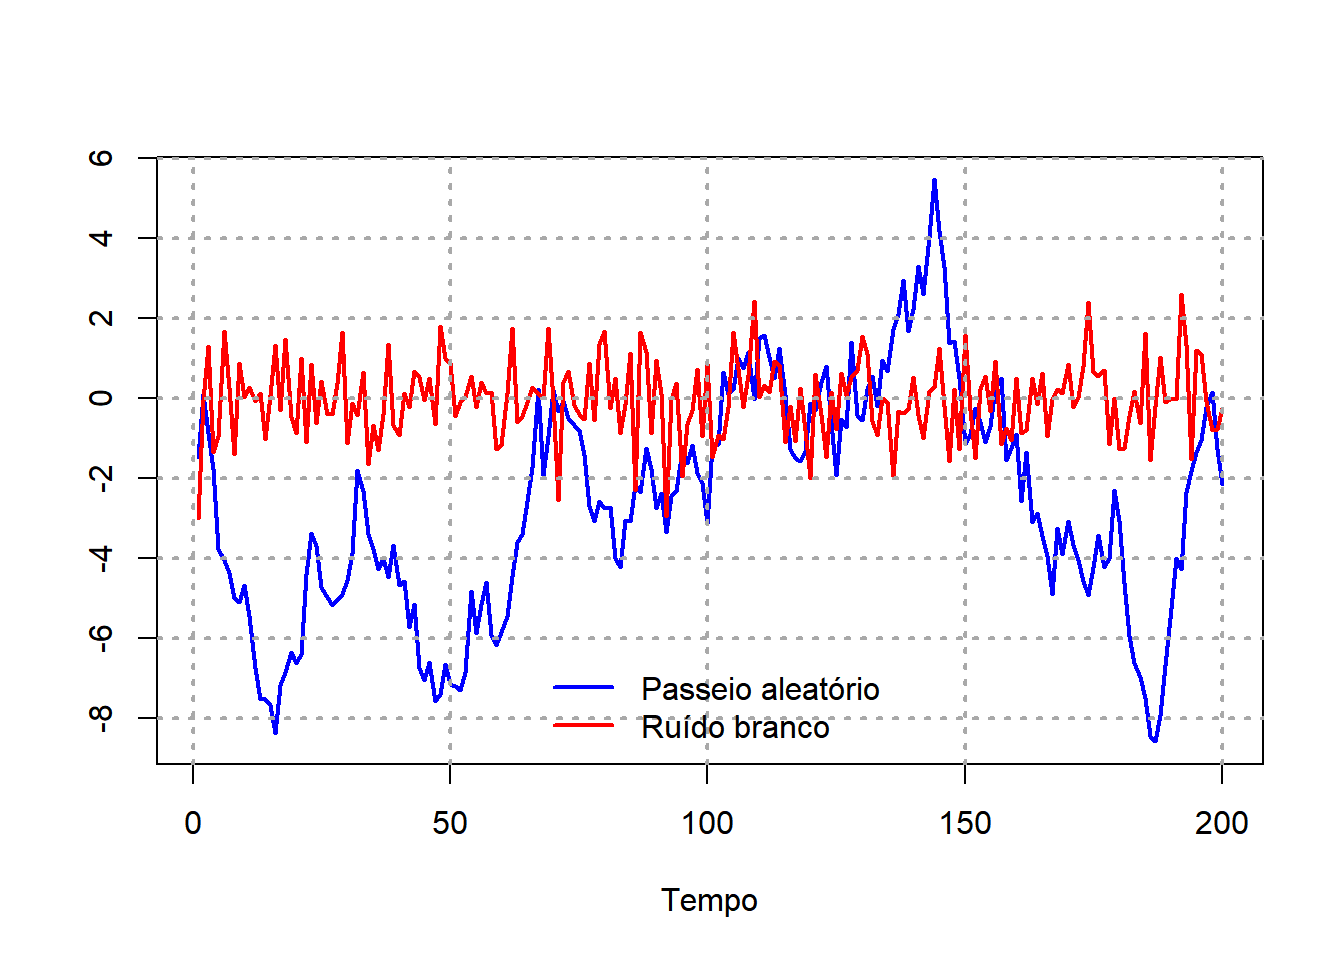
\includegraphics{Cap3_files/figure-latex/unnamed-chunk-13-1.pdf}

\begin{Shaded}
\begin{Highlighting}[]
\KeywordTok{plot}\NormalTok{(dados[,}\DecValTok{2}\NormalTok{])}
\NormalTok{mm_centrada_FP12 <-}\StringTok{ }\KeywordTok{ma}\NormalTok{(dados[,}\DecValTok{2}\NormalTok{],}\DataTypeTok{order=}\DecValTok{12}\NormalTok{)}
\KeywordTok{lines}\NormalTok{(mm_centrada_FP12,}\DataTypeTok{col=}\StringTok{"red"}\NormalTok{)}
\end{Highlighting}
\end{Shaded}

\includegraphics{Cap3_files/figure-latex/unnamed-chunk-13-2.pdf}

\begin{Shaded}
\begin{Highlighting}[]
\KeywordTok{plot}\NormalTok{(dados[,}\DecValTok{3}\NormalTok{])}
\NormalTok{mm_centrada_TD12 <-}\StringTok{ }\KeywordTok{ma}\NormalTok{(dados[,}\DecValTok{3}\NormalTok{],}\DataTypeTok{order=}\DecValTok{12}\NormalTok{)}
\KeywordTok{lines}\NormalTok{(mm_centrada_TD12,}\DataTypeTok{col=}\StringTok{"red"}\NormalTok{)}
\end{Highlighting}
\end{Shaded}

\includegraphics{Cap3_files/figure-latex/unnamed-chunk-13-3.pdf}

\#Média Móvel Simples \# z = Série temporal \# r = Tamanho \# l = Número

\begin{Shaded}
\begin{Highlighting}[]
\NormalTok{zDE <-}\StringTok{ }\NormalTok{dados[,}\DecValTok{1}\NormalTok{]}
\NormalTok{lDE <-}\StringTok{ }\DecValTok{15}
\NormalTok{rDE <-}\StringTok{ }\DecValTok{288}
\NormalTok{IC_DE <-}\StringTok{ }\ControlFlowTok{function}\NormalTok{(zDE,rDE,lDE)\{}
\NormalTok{smadfDE <-}\StringTok{ }\KeywordTok{SMA}\NormalTok{(zDE,rDE)}
\NormalTok{IC_IDE <-}\StringTok{ }\KeywordTok{rep}\NormalTok{(smadfDE[}\KeywordTok{length}\NormalTok{(zDE)],lDE) }\OperatorTok{-}\StringTok{ }\FloatTok{1.96}\OperatorTok{*}\KeywordTok{sd}\NormalTok{(zDE)}\OperatorTok{/}\KeywordTok{sqrt}\NormalTok{(rDE)}
\NormalTok{IC_SDE <-}\StringTok{ }\KeywordTok{rep}\NormalTok{(smadfDE[}\KeywordTok{length}\NormalTok{(zDE)],lDE) }\OperatorTok{+}\StringTok{ }\FloatTok{1.96}\OperatorTok{*}\KeywordTok{sd}\NormalTok{(zDE)}\OperatorTok{/}\KeywordTok{sqrt}\NormalTok{(rDE)}
\NormalTok{previsaoDE <-}\StringTok{ }\KeywordTok{rep}\NormalTok{(smadf[}\KeywordTok{length}\NormalTok{(zDE)],lDE)}
\KeywordTok{cbind}\NormalTok{(IC_IDE,previsaoDE,IC_SDE)}
\NormalTok{\}}


\NormalTok{zFP <-}\StringTok{ }\NormalTok{dados[,}\DecValTok{2}\NormalTok{]}
\NormalTok{lFP <-}\StringTok{ }\DecValTok{15}
\NormalTok{r <-}\StringTok{ }\DecValTok{288}
\NormalTok{IC_FP <-}\StringTok{ }\ControlFlowTok{function}\NormalTok{(zFP,rFP,lFP)\{}
\NormalTok{smadfFP <-}\StringTok{ }\KeywordTok{SMA}\NormalTok{(zFP,rFP)}
\NormalTok{IC_IFP <-}\StringTok{ }\KeywordTok{rep}\NormalTok{(smadfFP[}\KeywordTok{length}\NormalTok{(zFP)],l) }\OperatorTok{-}\StringTok{ }\FloatTok{1.96}\OperatorTok{*}\KeywordTok{sd}\NormalTok{(zFP)}\OperatorTok{/}\KeywordTok{sqrt}\NormalTok{(rFP)}
\NormalTok{IC_SFP <-}\StringTok{ }\KeywordTok{rep}\NormalTok{(smadfFP[}\KeywordTok{length}\NormalTok{(zFP)],l) }\OperatorTok{+}\StringTok{ }\FloatTok{1.96}\OperatorTok{*}\KeywordTok{sd}\NormalTok{(zFP)}\OperatorTok{/}\KeywordTok{sqrt}\NormalTok{(rFP)}
\NormalTok{previsaoFP <-}\StringTok{ }\KeywordTok{rep}\NormalTok{(smadfFP[}\KeywordTok{length}\NormalTok{(zFP)],lFP)}
\KeywordTok{cbind}\NormalTok{(IC_IFP,previsaoFP,IC_SFP)}
\NormalTok{\}}

\NormalTok{zTD <-}\StringTok{ }\NormalTok{dados[,}\DecValTok{3}\NormalTok{]}
\NormalTok{lTD <-}\StringTok{ }\DecValTok{15}
\NormalTok{rTD <-}\StringTok{ }\DecValTok{288}
\NormalTok{IC_TD <-}\StringTok{ }\ControlFlowTok{function}\NormalTok{(zTD,rTD,lTD)\{}
\NormalTok{smadfTD <-}\StringTok{ }\KeywordTok{SMA}\NormalTok{(zTD,rTD)}
\NormalTok{IC_ITD <-}\StringTok{ }\KeywordTok{rep}\NormalTok{(smadfTD[}\KeywordTok{length}\NormalTok{(zTD)],lTD) }\OperatorTok{-}\StringTok{ }\FloatTok{1.96}\OperatorTok{*}\KeywordTok{sd}\NormalTok{(zTD)}\OperatorTok{/}\KeywordTok{sqrt}\NormalTok{(rTD)}
\NormalTok{IC_STD <-}\StringTok{ }\KeywordTok{rep}\NormalTok{(smadfTD[}\KeywordTok{length}\NormalTok{(zTD)],lTD) }\OperatorTok{+}\StringTok{ }\FloatTok{1.96}\OperatorTok{*}\KeywordTok{sd}\NormalTok{(zTD)}\OperatorTok{/}\KeywordTok{sqrt}\NormalTok{(rTD)}
\NormalTok{previsaoTD <-}\StringTok{ }\KeywordTok{rep}\NormalTok{(smadfTD[}\KeywordTok{length}\NormalTok{(zTD)],lTD)}
\KeywordTok{cbind}\NormalTok{(IC_ITD,previsaoTD,IC_STD)}
\NormalTok{\}}
\end{Highlighting}
\end{Shaded}

Mostra a série suavizada que comeca no 12º mes. A previsão para os meses
futuros (última média móvel de um período de 12 meses).

\#Modelos de suavização exponencial \#Modelos para séries localmente
constantes \#Suavização exponencial simples(SES)

A previsão desse modelo é igual ao último valor exponencial suavizado
obtido.

\begin{Shaded}
\begin{Highlighting}[]
\NormalTok{serieDE =}\StringTok{ }\KeywordTok{ts}\NormalTok{(dados[,}\DecValTok{1}\NormalTok{],}\DataTypeTok{start =} \KeywordTok{c}\NormalTok{(}\DecValTok{1991}\NormalTok{,}\DecValTok{1}\NormalTok{),}\DataTypeTok{frequency =} \DecValTok{1}\NormalTok{)}
\NormalTok{serieFP =}\StringTok{ }\KeywordTok{ts}\NormalTok{(dados[,}\DecValTok{2}\NormalTok{],}\DataTypeTok{start =} \KeywordTok{c}\NormalTok{(}\DecValTok{2000}\NormalTok{,}\DecValTok{1}\NormalTok{),}\DataTypeTok{frequency =} \DecValTok{1}\NormalTok{)}
\NormalTok{serieTD =}\StringTok{ }\KeywordTok{ts}\NormalTok{(dados[,}\DecValTok{3}\NormalTok{],}\DataTypeTok{start =} \KeywordTok{c}\NormalTok{(}\DecValTok{1991}\NormalTok{,}\DecValTok{1}\NormalTok{),}\DataTypeTok{frequency =} \DecValTok{1}\NormalTok{)}
\end{Highlighting}
\end{Shaded}

\begin{Shaded}
\begin{Highlighting}[]
\NormalTok{ajusteDE<-}\KeywordTok{HoltWinters}\NormalTok{((serieDE), }\DataTypeTok{beta=}\OtherTok{FALSE}\NormalTok{, }\DataTypeTok{gamma=}\OtherTok{FALSE}\NormalTok{)}
\NormalTok{ajusteDE}
\end{Highlighting}
\end{Shaded}

\begin{verbatim}
## Holt-Winters exponential smoothing without trend and without seasonal component.
## 
## Call:
## HoltWinters(x = (serieDE), beta = FALSE, gamma = FALSE)
## 
## Smoothing parameters:
##  alpha: 0.9999497
##  beta : FALSE
##  gamma: FALSE
## 
## Coefficients:
##       [,1]
## a 800888.5
\end{verbatim}

\begin{Shaded}
\begin{Highlighting}[]
\NormalTok{ajusteFP<-}\KeywordTok{HoltWinters}\NormalTok{((serieFP), }\DataTypeTok{beta=}\OtherTok{FALSE}\NormalTok{, }\DataTypeTok{gamma=}\OtherTok{FALSE}\NormalTok{)}
\NormalTok{ajusteFP}
\end{Highlighting}
\end{Shaded}

\begin{verbatim}
## Holt-Winters exponential smoothing without trend and without seasonal component.
## 
## Call:
## HoltWinters(x = (serieFP), beta = FALSE, gamma = FALSE)
## 
## Smoothing parameters:
##  alpha: 0.2263615
##  beta : FALSE
##  gamma: FALSE
## 
## Coefficients:
##       [,1]
## a 269.2593
\end{verbatim}

\begin{Shaded}
\begin{Highlighting}[]
\NormalTok{ajusteTD<-}\KeywordTok{HoltWinters}\NormalTok{((serieTD), }\DataTypeTok{beta=}\OtherTok{FALSE}\NormalTok{, }\DataTypeTok{gamma=}\OtherTok{FALSE}\NormalTok{)}
\NormalTok{ajusteTD}
\end{Highlighting}
\end{Shaded}

\begin{verbatim}
## Holt-Winters exponential smoothing without trend and without seasonal component.
## 
## Call:
## HoltWinters(x = (serieTD), beta = FALSE, gamma = FALSE)
## 
## Smoothing parameters:
##  alpha: 0.9999339
##  beta : FALSE
##  gamma: FALSE
## 
## Coefficients:
##       [,1]
## a 12.49999
\end{verbatim}

\begin{Shaded}
\begin{Highlighting}[]
\KeywordTok{plot}\NormalTok{(ajusteDE)}
\end{Highlighting}
\end{Shaded}

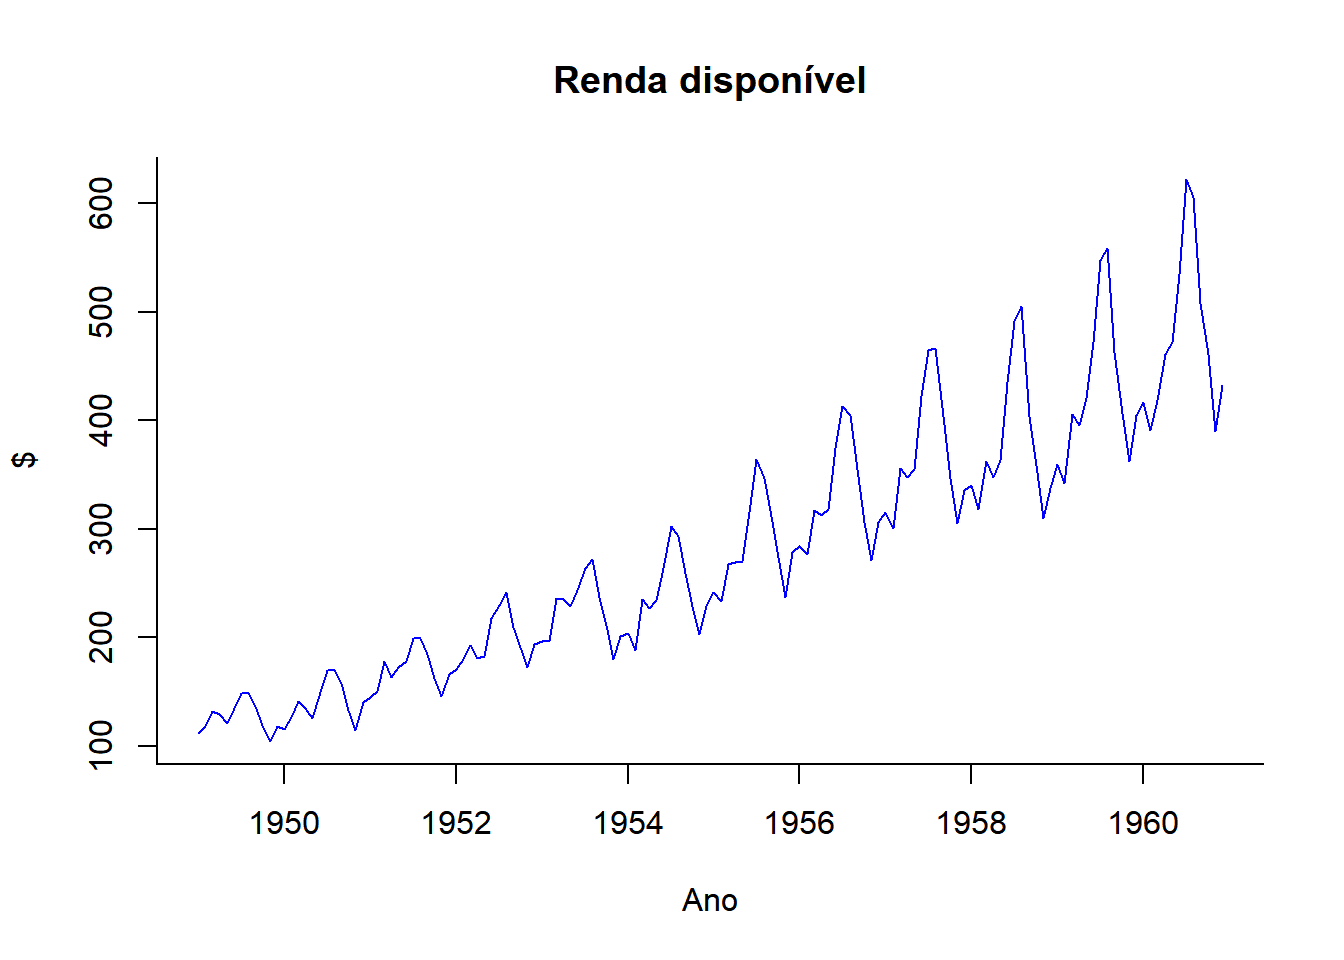
\includegraphics{Cap3_files/figure-latex/unnamed-chunk-18-1.pdf}

\begin{Shaded}
\begin{Highlighting}[]
\KeywordTok{plot}\NormalTok{(ajusteFP)}
\end{Highlighting}
\end{Shaded}

\includegraphics{Cap3_files/figure-latex/unnamed-chunk-18-2.pdf}

\begin{Shaded}
\begin{Highlighting}[]
\KeywordTok{plot}\NormalTok{(ajusteTD)}
\end{Highlighting}
\end{Shaded}

\includegraphics{Cap3_files/figure-latex/unnamed-chunk-18-3.pdf}

\#Modelo para séries com tendência Suavização exponencial de Holt (SEH)

\begin{Shaded}
\begin{Highlighting}[]
\NormalTok{ajuste_com_tendenciaDE<-}\KeywordTok{HoltWinters}\NormalTok{(dados[,}\DecValTok{1}\NormalTok{], }\DataTypeTok{gamma=}\OtherTok{FALSE}\NormalTok{)}
\NormalTok{ajuste_com_tendenciaDE}
\end{Highlighting}
\end{Shaded}

\begin{verbatim}
## Holt-Winters exponential smoothing with trend and without seasonal component.
## 
## Call:
## HoltWinters(x = dados[, 1], gamma = FALSE)
## 
## Smoothing parameters:
##  alpha: 1
##  beta : 0.203323
##  gamma: FALSE
## 
## Coefficients:
##         [,1]
## a 800889.430
## b   8053.882
\end{verbatim}

\begin{Shaded}
\begin{Highlighting}[]
\NormalTok{ajuste_com_tendenciaFP<-}\KeywordTok{HoltWinters}\NormalTok{(dados[,}\DecValTok{2}\NormalTok{], }\DataTypeTok{gamma=}\OtherTok{FALSE}\NormalTok{)}
\NormalTok{ajuste_com_tendenciaFP}
\end{Highlighting}
\end{Shaded}

\begin{verbatim}
## Holt-Winters exponential smoothing with trend and without seasonal component.
## 
## Call:
## HoltWinters(x = dados[, 2], gamma = FALSE)
## 
## Smoothing parameters:
##  alpha: 0.2155786
##  beta : 0.009025177
##  gamma: FALSE
## 
## Coefficients:
##          [,1]
## a 269.6699512
## b   0.5435858
\end{verbatim}

\begin{Shaded}
\begin{Highlighting}[]
\NormalTok{ajuste_com_tendenciaTD<-}\KeywordTok{HoltWinters}\NormalTok{(dados[,}\DecValTok{3}\NormalTok{], }\DataTypeTok{gamma=}\OtherTok{FALSE}\NormalTok{)}
\NormalTok{ajuste_com_tendenciaTD}
\end{Highlighting}
\end{Shaded}

\begin{verbatim}
## Holt-Winters exponential smoothing with trend and without seasonal component.
## 
## Call:
## HoltWinters(x = dados[, 3], gamma = FALSE)
## 
## Smoothing parameters:
##  alpha: 1
##  beta : 0.8882952
##  gamma: FALSE
## 
## Coefficients:
##           [,1]
## a 12.500000000
## b  0.009864207
\end{verbatim}

\begin{Shaded}
\begin{Highlighting}[]
\KeywordTok{plot}\NormalTok{(dados[,}\DecValTok{1}\NormalTok{])}
\KeywordTok{lines}\NormalTok{(}\KeywordTok{fitted}\NormalTok{(ajuste_com_tendenciaDE)[,}\DecValTok{1}\NormalTok{],}\DataTypeTok{col=}\StringTok{"red"}\NormalTok{,}\DataTypeTok{lty=}\DecValTok{2}\NormalTok{,}\DataTypeTok{lwd =}\DecValTok{3}\NormalTok{)}
\KeywordTok{legend}\NormalTok{(}\StringTok{'topleft'}\NormalTok{, }\DataTypeTok{legend=}\KeywordTok{c}\NormalTok{(}\StringTok{"Depositos em poupança"}\NormalTok{, }\StringTok{"ajuste_com_tendencia"}\NormalTok{),}\DataTypeTok{bty =} \StringTok{"n"}\NormalTok{,}
       \DataTypeTok{col=}\KeywordTok{c}\NormalTok{(}\StringTok{"black"}\NormalTok{,}\StringTok{"red"}\NormalTok{), }\DataTypeTok{lty=}\KeywordTok{c}\NormalTok{(}\DecValTok{1}\NormalTok{,}\DecValTok{2}\NormalTok{), }\DataTypeTok{cex=}\FloatTok{0.8}\NormalTok{,}\DataTypeTok{lwd =}\KeywordTok{c}\NormalTok{(}\DecValTok{1}\NormalTok{,}\DecValTok{3}\NormalTok{))}
\end{Highlighting}
\end{Shaded}

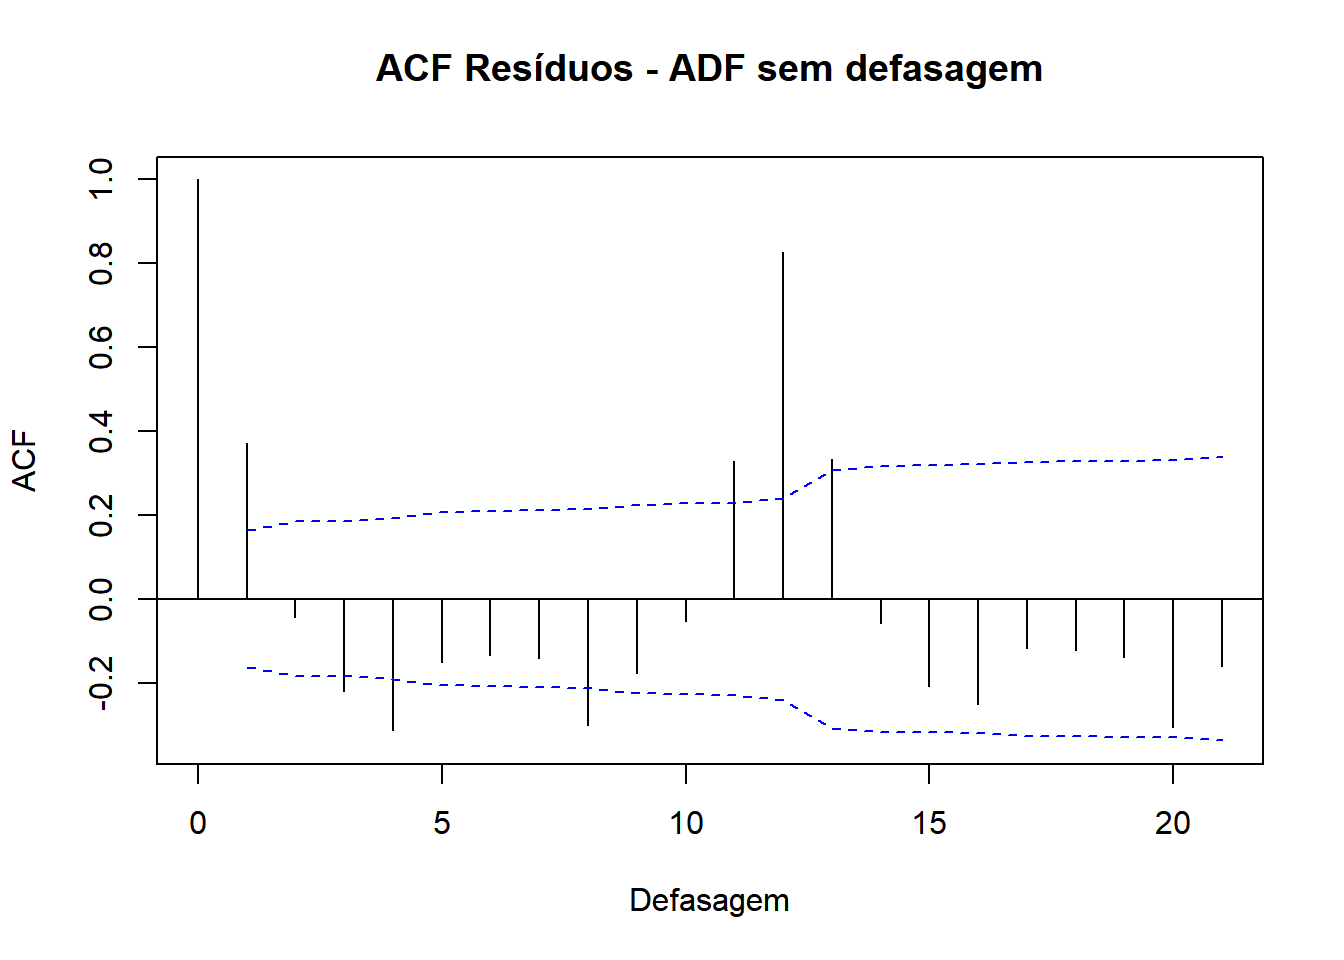
\includegraphics{Cap3_files/figure-latex/unnamed-chunk-21-1.pdf}

\begin{Shaded}
\begin{Highlighting}[]
\KeywordTok{plot}\NormalTok{(dados[,}\DecValTok{2}\NormalTok{])}
\KeywordTok{lines}\NormalTok{(}\KeywordTok{fitted}\NormalTok{(ajuste_com_tendenciaFP)[,}\DecValTok{1}\NormalTok{],}\DataTypeTok{col=}\StringTok{"red"}\NormalTok{,}\DataTypeTok{lty=}\DecValTok{2}\NormalTok{,}\DataTypeTok{lwd =}\DecValTok{3}\NormalTok{)}
\KeywordTok{legend}\NormalTok{(}\StringTok{'topleft'}\NormalTok{, }\DataTypeTok{legend=}\KeywordTok{c}\NormalTok{(}\StringTok{"Folha de Pagamentos"}\NormalTok{, }\StringTok{"ajuste_com_tendencia"}\NormalTok{),}\DataTypeTok{bty =} \StringTok{"n"}\NormalTok{,}
       \DataTypeTok{col=}\KeywordTok{c}\NormalTok{(}\StringTok{"black"}\NormalTok{,}\StringTok{"red"}\NormalTok{), }\DataTypeTok{lty=}\KeywordTok{c}\NormalTok{(}\DecValTok{1}\NormalTok{,}\DecValTok{2}\NormalTok{), }\DataTypeTok{cex=}\FloatTok{0.8}\NormalTok{,}\DataTypeTok{lwd =}\KeywordTok{c}\NormalTok{(}\DecValTok{1}\NormalTok{,}\DecValTok{3}\NormalTok{))}
\end{Highlighting}
\end{Shaded}

\includegraphics{Cap3_files/figure-latex/unnamed-chunk-21-2.pdf}

\begin{Shaded}
\begin{Highlighting}[]
\KeywordTok{plot}\NormalTok{(dados[,}\DecValTok{3}\NormalTok{])}
\KeywordTok{lines}\NormalTok{(}\KeywordTok{fitted}\NormalTok{(ajuste_com_tendenciaTD)[,}\DecValTok{1}\NormalTok{],}\DataTypeTok{col=}\StringTok{"red"}\NormalTok{,}\DataTypeTok{lty=}\DecValTok{2}\NormalTok{,}\DataTypeTok{lwd =}\DecValTok{3}\NormalTok{)}
\KeywordTok{legend}\NormalTok{(}\StringTok{'topleft'}\NormalTok{, }\DataTypeTok{legend=}\KeywordTok{c}\NormalTok{(}\StringTok{"Taxa de desemprego"}\NormalTok{, }\StringTok{"ajuste_com_tendencia"}\NormalTok{),}\DataTypeTok{bty =} \StringTok{"n"}\NormalTok{,}
       \DataTypeTok{col=}\KeywordTok{c}\NormalTok{(}\StringTok{"black"}\NormalTok{,}\StringTok{"red"}\NormalTok{), }\DataTypeTok{lty=}\KeywordTok{c}\NormalTok{(}\DecValTok{1}\NormalTok{,}\DecValTok{2}\NormalTok{), }\DataTypeTok{cex=}\FloatTok{0.8}\NormalTok{,}\DataTypeTok{lwd =}\KeywordTok{c}\NormalTok{(}\DecValTok{1}\NormalTok{,}\DecValTok{3}\NormalTok{))}
\end{Highlighting}
\end{Shaded}

\includegraphics{Cap3_files/figure-latex/unnamed-chunk-21-3.pdf}

\#Modelo para séries sazonais \#Suavização exponencial de Holt-Winters
(HW) \#Modelo Aditivo \#Modelo Multiplicativo

O HW ajuda a descobrir padrão de comportamento mais complexos. A
previsão desse modelo é feita de acordo com a série que pode ser Sazonal
Aditiva ou Sazonal Multiplicativa.

\begin{Shaded}
\begin{Highlighting}[]
\NormalTok{ajuste_com_sazonalidade<-}\KeywordTok{HoltWinters}\NormalTok{(AirPassengers)}
\NormalTok{ajuste_com_sazonalidade}
\end{Highlighting}
\end{Shaded}

\begin{verbatim}
## Holt-Winters exponential smoothing with trend and additive seasonal component.
## 
## Call:
## HoltWinters(x = AirPassengers)
## 
## Smoothing parameters:
##  alpha: 0.2479595
##  beta : 0.03453373
##  gamma: 1
## 
## Coefficients:
##           [,1]
## a   477.827781
## b     3.127627
## s1  -27.457685
## s2  -54.692464
## s3  -20.174608
## s4   12.919120
## s5   18.873607
## s6   75.294426
## s7  152.888368
## s8  134.613464
## s9   33.778349
## s10 -18.379060
## s11 -87.772408
## s12 -45.827781
\end{verbatim}

\begin{Shaded}
\begin{Highlighting}[]
\KeywordTok{plot}\NormalTok{(AirPassengers)}
\KeywordTok{lines}\NormalTok{(}\KeywordTok{fitted}\NormalTok{(ajuste_com_sazonalidade)[,}\DecValTok{1}\NormalTok{],}\DataTypeTok{col=}\StringTok{"red"}\NormalTok{,}\DataTypeTok{lty=}\DecValTok{2}\NormalTok{,}\DataTypeTok{lwd =}\DecValTok{3}\NormalTok{)}
\KeywordTok{legend}\NormalTok{(}\StringTok{'topleft'}\NormalTok{, }\DataTypeTok{legend=}\KeywordTok{c}\NormalTok{(}\StringTok{"AirPassengers"}\NormalTok{, }\StringTok{"ajuste_com_sazonalidade"}\NormalTok{),}
  \DataTypeTok{bty =} \StringTok{"n"}\NormalTok{,}\DataTypeTok{col=}\KeywordTok{c}\NormalTok{(}\StringTok{"black"}\NormalTok{,}\StringTok{"red"}\NormalTok{), }\DataTypeTok{lty=}\KeywordTok{c}\NormalTok{(}\DecValTok{1}\NormalTok{,}\DecValTok{2}\NormalTok{), }\DataTypeTok{cex=}\FloatTok{0.8}\NormalTok{,}\DataTypeTok{lwd =}\KeywordTok{c}\NormalTok{(}\DecValTok{1}\NormalTok{,}\DecValTok{3}\NormalTok{))}
\end{Highlighting}
\end{Shaded}

\includegraphics{Cap3_files/figure-latex/unnamed-chunk-24-1.pdf}

```


\end{document}
